\section{CC Transformation}
\label{sec:cc_transform}

As shown in \Cref{sec:ioc_rules}, almost all IoC SCFs considered, except for $\RP_i$ and $\UCg$, fail CC. Out of these two, $\RP_i$ violates anonymity, and $\UCg$ selects a unique winner only if there is a Condorcet winner ($|\Sm(\profile)|=1$) \citep{Holliday23:Split}, implying it is not decisive for any $\profile$ without this property. As both anonymity and decisiveness are fundamental properties for SCFs (for ensuring the result is fair and conclusive, respectively), having CC rules that also satisfy them would be desirable, especially considering the strong guarantees of CC against strategic behavior, which we will further discuss in \Cref{sec:oioc}. To this end, we show that any neutral SCF can be efficiently modified to satisfy CC, while preserving its desirable properties, including anonymity and decisiveness, among others.

\subsection{Background: Clone Structures and PQ-Trees}\label{subsec:pqtrees}
For a profile $\profile$, \citet{Elkind10:Clone} define the \emph{clone structure} $\family(\profile) \subseteq \mathcal{P}(\cand)$ as the family of \textit{all} clone sets with respect to $\profile$. For example, for $\profile$ from Fig.~\ref{fig:eg_prof}, $\family(\profile)=\{\{a\},\{b\}, \{c\}, \{d\}, \{b,c\}, \{a,b,c,d\}\}$. They identify two types of \emph{irreducible} clone structures: a \emph{maximal} clone structure (also called a \emph{string of sausages}) and a \emph{minimal} clone structure (also called a \emph{fat sausage}). A string of sausages arises when each ranking in  $\profile$ is either a fixed linear order (say, $\sigma_1 : a_1 \succ a_2 \succ \cdots \succ a_m$) or its reversal. In this case, $\family(\profile) = \{ \{a_k\}_{i\le k\le j}: i\le j\}$, \emph{i.e.}, all intervals in $\sigma_1$. The \emph{majority ranking} of the string of sausages is $\sigma_1$ or its reverse, depending on which one appears more frequently in $\profile$. A fat sausage occurs when $\family(\profile) = \{A\} \cup \{\{a_i\}\}_{i \in [m]}$, \emph{i.e.}, the structure only has the trivial clone sets. 

Our CC transformation uses \emph{PQ-trees}: a data structure first defined by \citet{Booth76:Testing} and later used by \citet{Elkind10:Clone} to represent clone sets.
Here, we present the definitions required for our construction; for the full treatment, see \citet{Elkind10:Clone}
(and our \Cref{subsec:extended_pqtrees}).

A {\em PQ-tree} $T$ over $\cand$ is an ordered tree whose leaves correspond to the elements of $\cand$. To represent a clone structure $\family(\profile)$ as a PQ-tree, we iteratively identify irreducible subfamilies of $\family(\profile)$, and collapse them into a single meta-candidate. 
If the subfamily corresponds to a fat sausage, we group its members under an internal node of type P, denoted as a $\odot$-product of its children.
On the other hand, if the subfamily corresponds to a string of sausages, we group its members under an internal node of type Q, denoted as a $\oplus$-product of its children. 
In rankings compatible with $\family(\profile)$, the children of a P-node can be permuted arbitrarily; the order of the children of a Q-node must follow its majority ranking or its reversal. Crucially, the order of collapsing is not important, as the irreducible subfamilies of a clone structure are non-overlapping \cite[Prop. 4.2.]{Elkind10:Clone}. 

\begin{example}\label{ex:pq-tree}
    Let $\profile$ be a profile on $A=\{a, b, c, d\}$ with two rankings: $a\succ b \succ c \succ d$ and $d \succ c \succ a \succ b$.
    Then, $\family(\profile) = \{\{a\}, \{b\}, \{c\}, \{d\}, \{a,b\}, \{c, d\}, \{a, b, c\}, A\}$.
    Collapsing the irreducible subfamily $K_1 = \{a, b\}$, the updated $\family(\profile)$  is $\{\{c\}, \{d\}, \{K_1\}, \{c, d\}, \{K_1, c\}, \{K_1, c, d\}\}$.
    With size two, $K_1$ is both a string of sausages and a fat sausage; by convention we treat it as a fat sausage (\emph{i.e.}, of type \emph{P}).
    The updated $\family(\profile)$ is a string of sausages itself, so the algorithm terminates by picking the root of the tree as a type \emph{Q} node. The resulting PQ-tree is illustrated in \Cref{fig:tree} (left).
    
    \begin{figure}[t]
        \centering
        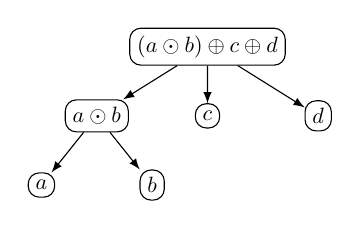
\begin{tikzpicture}
            [
              grow=down,
              sibling distance=4em,
              level distance=2.5em,
              edge from parent/.style={draw, -latex},
              every node/.style={draw, rectangle, rounded corners, align=center, scale=0.8}
            ]
            \node {$(a \odot b) \oplus c \oplus d$}
              child { node {$a \odot b$}
                child { node {$a$} }
                child { node {$b$} }
              }
              child { node {$c$} }
              child { node {$d$} };
        \end{tikzpicture} \quad \quad \quad \quad
        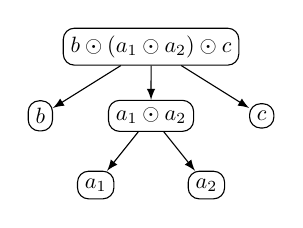
\begin{tikzpicture}
            [
              grow=down,
              sibling distance=4em,
              level distance=2.5em,
              edge from parent/.style={draw, -latex},
              every node/.style={draw, rectangle, rounded corners, align=center, scale=0.8}
            ]
            \node {$b\odot (a_1 \odot a_2) \odot c$}
              child { node {$b$} }
              child { node {$a_1 \odot a_2$}
                child { node {$a_1$} }
                child { node {$a_2$} }
              }
              child { node {$c$} };
        \end{tikzpicture}
        \caption{(Left) The PQ-tree representing $\family(\profile)$ from  \Cref{ex:pq-tree} . (Right) The PQ-tree of $\profile$ from \Cref{fig:bg_eg}.}\label{fig:tree}
    \end{figure}
\end{example}

We now formulate two useful properties of PQ-trees, as observed by 
\citet{Cornaz13:Kemeny}.

\begin{restatable}[\citealt{Cornaz13:Kemeny}]{lemma}{pqpoly} \label{lemma:pq-poly}
    PQ-trees can be constructed in $O(|\voter|\cdot|\cand|^3)=O(nm^3)$ time.
\end{restatable}

\begin{restatable}[{\citealt[Prop. 4]{Cornaz13:Kemeny}}]{lemma}{pqclones} \label{lemma:pq_clones}
    Given $\profile$ and its PQ-tree $T$, a set of candidates $K \subseteq A$ is a clone set if and only if it satisfies one of the following: (1) $K$ exactly corresponds to the leaves of a subtree in $T$ (where leaves are also subtrees of size 1), or (2) $K$ exactly corresponds to the leaves of a set of subtrees the roots of which are adjacent descendants of a Q-node in $T$. 
\end{restatable}

\citet{Cornaz13:Kemeny} use PQ-trees to prove fixed-parameter tractability of computing a \emph{Kemeny ranking} of a profile, which obeys a special case of CC (see \Cref{sec:spf} for CC properties of social preference functions, which return aggregate rankings over $\cand$ rather than subsets). Similarly, \citet{Brandt11:Fixed} show that any CC tournament solution is fixed-parameter tractable with respect to the properties of an analogous construct for tournaments (decomposition trees) by running the TS recursively on the nodes of the tree.\footnote{A similar idea of breaking the computation into subsets of candidates is used by \citet{Conitzer06:Computing} for computing Slater rankings of a profile. The eligible subsets in this case (which the author simply refers to as sets of \emph{similar candidates}) exactly correspond to the components of the tournament induced by the profile (see our \Cref{appdef:component_tour}).} Our key observation is that even if we start with an SCF that does \emph{not} satisfy CC (or any weaker version thereof), running it on the PQ-tree enables us to define a \emph{new} SCF that is in fact CC, while maintaining many desirable properties of the original SCF. In the following section, we introduce this transformation and formalize its properties.

\subsection{CC-Transformed SCFs}\label{subsec:transform}
We now present Algorithm~\ref{alg:cc-transform}, which is based on a similar algorithm by \citet{Brandt11:Fixed} for efficiently implementing CC tournament solutions. Given $T=PQ(\profile)$ (the PQ-tree for a profile $\profile$), we refer to its nodes by the subset of candidates in their subtrees. For $\node \subseteq \cand$, is\_p\_node($\node,T$) returns True (resp., False) if the node corresponding to $B$ in $T$ is a P- (resp., Q-) node, raising an error if no such node exists. Let decomp($\node,T$) return the clone decomposition $\decomp$ corresponding to node $\node$, where each $K\in \mathcal{K}$ is a child node of $\node$ (these are clone sets by Lemma~\ref{lemma:pq_clones}).
For example, if $T$ is the tree from Fig.~\ref{fig:tree}(left),
decomp($A,T)=\{\{a,b\}, \{c\}, \{d\}\}$ and  decomp($\{a,b\},T)=\{\{a\}, \{b\}\}$.  For a Q-node $\node$, let $\node_i(\node,T)$ be the $i$-th child of $\node$ according to its majority ranking $\sigma_1$. 

\begin{definition}\label{def:cc-transform}
    Given an SCF $f$, the \emph{CC-transform} of $f$ is an SCF $f^{CC}$ that, on input profile $\boldsymbol{\sigma}$, outputs the candidates consistent with the output of Algorithm~\ref{alg:cc-transform} on input $f$ and $\boldsymbol{\sigma}$. 
\end{definition}

Intuitively, $f^{CC}$ recursively runs $f$ on the PQ-tree of $\profile$, starting at the root. At every P-node $B$, $f^{CC}$ runs $f$ on the summary induced by that node ($\profile^{\text{decomp($\node,T$)}}$), and continues with the winner children. At every Q-node $\node$, it runs $f$ on the summary of the node \emph{restricted} to its first two child nodes ($B_1(\node,T)$ and $B_2(\node,T)$). If the winner is $B_1(\node,T)$ (resp., $B_2(\node,T)$), it continues with the first (resp., last) child node of $\node$, \emph{i.e.}, $B_1(\node, T)$ (resp, $B_{|\text{decomp($\node,T$)}|}(\node, T)$); if both are winners, then $f$ continues with \emph{all} the children of $\node$. The intuition for this is that for any Q-node $\node$ of $T$, the pairwise relationship between $B_i(\node,T)$ and $B_j(\node,T)$ is the same for all $i<j$, so if $B_1(\profile, \decomp)$ defeats $B_2(\profile, \decomp)$ according to $f$ (in a pairwise comparison), it will also defeat $B_j(\profile, \decomp)$ for any $j>1$ by the neutrality of $f$. If $B_2(\profile, \decomp)$ defeats $B_1(\profile, \decomp)$ according to $f$, on the other hand, then $B_j(\profile, \decomp)$ will defeat $B_i(\profile, \decomp)$ for any $j>i$ by the neutrality of $f$, naturally leading us to the last child node, $B_{|\text{decomp($\node,T$)}|}(\node, T)$. Lastly, if both $B_1(\profile, \decomp)$ and $B_2(\profile, \decomp)$ are winners, this implies $f$ cannot choose between any pair of child nodes of $\node$, which is why we continue with all child nodes.


\begin{algorithm}[t]
    \caption{CC transformation for SCF}\label{alg:cc-transform}
    \SetAlgoNoLine
    \KwIn{SCF $f$, preference profile $\boldsymbol{\sigma}$ over candidates $\cand$}
    \KwOut{Winner candidates $W \subseteq \cand$}
    $W =\emptyset$  \tcp*{Winner list, initialized as empty}
    $T = PQ(\profile)$\tcp*{Constructs the PQ-tree for $\profile$}
    $\queue = (\cand)$ \tcp*{Queue of nodes, starting with root node}
    \While{$|\queue| \neq 0$}{
        $\node =$ Dequeue($\queue$)\;
        \eIf(\tcp*[f]{$\node$ is a leaf node}){$|\node|=1$}{
            $W = W \cup \node$ \tcp*{Add $B$ to list of winners}}{
            $\decomp =$decomp$(\node,T)$\ \tcp*{Each $B' \in \decomp$ is a child node of $\node$}
            \uIf(\tcp*[f]{$\node$ is a P-node}){is\_p\_node$(\node,T)$}{
                \lFor(\tcp*[f]{Run $f$ on summary, enqueue winners}){$K \in f(\profile^\mathcal{K})$}{Enqueue($\queue,K$)}
            }
            \Else(\tcp*[f]{$\node$ is a Q-node}){
                $W'=f(\profile^\mathcal{K})|_{\{\node_1(\node,T),\node_2(\node,T)\}}$ \tcp*{Run $f$ on the first two child nodes}
                \uIf{$W'=\{\node_1(\node,T)\}$}{Enqueue($\queue,\node_1(\node,T)$)\tcp*[f]{Enqueue the first child of $B$}}
                \uElseIf{$W'=\{\node_2(\node,T)\}$}{Enqueue($\queue,\node_{|\decomp|}(\node,T)$)\tcp*[f]{Enqueue the last child of $B$}}
                \Else(\tcp*[f]{$W'=\{\node_1(\node,T),\node_2(\node,T)\}$}){
                    \lFor(\tcp*[f]{Enqueue \emph{all} children of $B$}){$K \in \decomp$}{Enqueue($\queue,K$)}
                }

            }

            }
        }
\end{algorithm}


We will shortly show that $f^{CC}$ satisfies CC, even if $f$ fails it. Of course, a useless transformation like $f^{CC'}(\profile)=\cand$ for all $\profile$ would also achieve this. As such, we want to show that $f^{CC}$ \textit{preserves} some of $f$'s desirable properties. It is straightforward to see that anonymity and neutrality are preserved, as \Cref{alg:cc-transform} is robust to relabeling of candidates and/or voters. Further, as we will show, Condorcet and Smith consistency, as well as decisiveness, are among the preserved properties.


Unfortunately, $f^{CC}$ does not preserve monotonicity, independence of Smith-dominated alternatives (ISDA), or participation. This is since changing an existing vote or adding a new candidate/voter can alter the clone structure of $\profile$, and thus its PQ-tree. We introduce relaxations of these axioms that require robustness against changes that \textit{respect} the clone structure. We first define the relaxation of monotonicity. 
\begin{restatable}{definition}{camono}\label{def:weak-mono}
    An SCF $f$ satisfies \emph{clone-aware monotonicity (monotonicity$\ca$)} if $a \in f(\profile)$ implies $a \in f(\profile')$ whenever (1) $\family(\profile)=\family(\profile')$ and (2) for all $i \in N$ and $b,c \in A \setminus\{a\}$, we have $a \succ_{\sigma_i} b \Rightarrow a \succ_{\sigma'_i} b$ and $b \succ_{\sigma_i} c \Rightarrow b \succ_{\sigma'_i} c$.
\end{restatable}
The only difference between Definition~\ref{def:weak-mono} and the usual definition of monotonicity (\emph{i.e.}, promoting a winner in some votes while keeping all else constant should not cause them to lose) is the requirement that $\profile$ and $\profile'$ have the same clone structure. ISDA$\ca$ and participation$\ca$ are defined analogously; see \Cref{appsec:ca-axioms} for formal definitions and examples showing why we need these relaxations. These new axioms implicitly assume that clone structures are \textit{inherent}, based on candidates' location in some shared perceptual space (in line with the original interpretation by \citet{Tideman87:Independence}), so any ``realistic'' change to $\profile$ will not alter its clone sets.

Lastly, in order to analyze the computational complexity of $f^{CC}$, we introduce the \emph{decomposition degree} of a tree, which we adapt from the definition of the decomposition degree of a tournament introduced by \citet{Brandt11:Fixed} in their study of CC tournament solutions. 
Following their fixed-parameter tractability framework, we will state the runtime of \Cref{alg:cc-transform} in terms of a parameter $\delta$ (which corresponds to the decomposition degree of a PQ-tree, formalized below in \Cref{def:delta}) and the running time of the input SCF $f$. 

\begin{definition}\label{def:delta}
    Given a PQ-tree $T$ for a profile $\profile$, let $\mathcal{P}$ denote the set of P-nodes in $T$. 
    The \emph{decomposition degree} $\delta(T)$ of the PQ-tree $T$ is defined as
    \begin{align*}
        \delta(T)= 
        \begin{cases}
            \max_{\node \in \mathcal{P}} |\text{decomp}(\node,T)| & \mathrm{ if } \, \mathcal{P} \neq \emptyset, \\ 
            2 & \mathrm{otherwise}.
        \end{cases}
    \end{align*}
\end{definition}
Intuitively, $\delta(T)$ is the maximum number of candidates with which \Cref{alg:cc-transform} will run $f$, \emph{e.g.}, in the two PQ-trees from \Cref{fig:tree}, $\delta(T)=3$. We now present our main result on CC-transforms.

\begin{restatable}{theorem}{cctransform} \label{thm:cc_transform}
    For any neutral SCF $f$, $f^{CC}$ satisfies:
    \begin{enumerate}[label={(\arabic*)}]
        \item If $\boldsymbol{\sigma}$ has no non-trivial clone sets, $f^{CC}(\boldsymbol{\sigma})=f(\boldsymbol{\sigma})$.
        \item $f^{CC}$ is composition-consistent.
        \item If $f$ is composition-consistent, then $f^{CC}=f$, \emph{i.e.}, they agree for all $\profile$.
        \item If $f$ satisfies any of \{anonymity, Condorcet consistency, Smith consistency, decisiveness (on all $\profile$), monotonicity$\ca$, ISDA$\ca$, participation$\ca$\}, then $f^{CC}$ satisfies this property as well.
        \item Let $g(n, m)$ be an upper bound on the runtime of an algorithm that computes $f$ on profiles with $n$ voters and $m$ candidates; then, $f^{CC}(\profile)$ can be computed in time $O(nm^3) + m \cdot g(n, \delta(PQ(\profile)))$.
    \end{enumerate}
\end{restatable}

\noindent Taken together, (2) and (3) immediately imply that our CC transformation is idempotent.
\begin{corollary}
    For any neutral SCF $f$, we have $(f^{CC})^{CC}=f^{CC}$, \emph{i.e.}, they agree for all $\profile$.
\end{corollary}

\noindent Further, (5) from \Cref{thm:cc_transform} implies that our CC-transform preserves efficient computability. 
\begin{corollary}
    If $f$ is polynomial-time computable, then so is $f^{CC}$.
\end{corollary}

Even if $f$ is not polynomial-time computable, (5) in \Cref{thm:cc_transform} gives us a running time that depends on the decomposition degree $\delta(T)$ of the PQ-tree. Therefore, we have shown a stronger result: namely, we obtain fixed-parameter tractability for $f^{CC}$ (in terms of $\delta(T)$) for all (neutral) SCFs $f$ with runtime that is polynomial in $n$. 
For example, this includes SCFs that are \NP-hard to compute when the number of candidates $m$ is arbitrarily large, but is polynomial-time computable for constant $m$. Indeed, as mentioned in \Cref{subsec:rp}, a well-known SCF that falls in this category is (anonymous) $RP$ \citep{Brill12:Price}.
Moreover, by (3) in \Cref{thm:cc_transform}, fixed-parameter tractability holds not just for the CC-transform $f^{CC}$ of any (neutral) SCF $f$, but also for all SCFs that are CC to begin with. 

Despite the above theoretical guarantees of \Cref{alg:cc-transform} regarding tractability and axiomatic properties, one can still question how useful our CC-transform is \emph{in practice}, as it does not modify the SCF unless actual clone sets exist (by (1) of \Cref{thm:cc_transform}). While clone sets are unlikely in political elections (where the number of candidates is reasonably bounded anyway), they may easily occur in settings where candidates or voters are not human. For example, if the candidates are AI outputs---\emph{e.g.}, for reinforcement learning from human feedback (RLHF)---it is relatively easy to introduce minorly tweaked versions of the same output into the evaluation process (see \Cref{sec:disc} for a discussion of why our results may be highly relevant for RLHF). Further, voters too could be not human~\citep{Xu24:Aggregating}. For example, if voters are benchmarks against which we are testing AI models (and we are supposed to choose a model by aggregating the ranking resulting from each benchmark) \citep{Lanctot25:Evaluating}, variants of the same model are likely to have similar performance on each benchmark. More classically, meta-search engines aggregate results from various ranking algorithms, each of which plays the role of a voter \citep{Dwork01:Rank}, and cloned webpages are likely to be ranked together by each algorithm. The guarantees of \Cref{thm:cc_transform} can be even more critical in settings such as these, as (a) the cost of cloning can be arbitrarily low, making it all the more important that the SCF used cannot be manipulated by such clones, and (b) the number of candidates can be very large due to such cloning, making tractability a significant concern.

Before ending our discussion of CC-transforms, it is worth comparing $f^{CC}$ to two similar notions from prior literature. First, in addition to CC, \citet{Laffond96:Composition} defined the \textit{CC hull} of an SCF $f$: the smallest (by inclusion) CC solution containing $f$. However, the CC hull does not necessarily preserve Condorcet consistency and achieves CC by adding candidates to the returned set, which sacrifices decisiveness. Second, in an unpublished preprint, \citet{Heitzig02:Social} introduces a similar recurrent CC transformation for SCFs. However, his transformation does not specify the order in which clone sets need to be collapsed and requires the original SCF to satisfy additional axioms, including Condorcet consistency and anonymity.

